\chapter{Combining data from individual stations}
\label{ch:cluster}


\section{Extensive air showers triggering multiple stations}

Each detection station samples air showers using the scintillator detectors. If a station pair is within \SI{2e3}{\meter} of each other they can detect the same showers. If the stations are closer together the rate of coincidences increases because the sensitivity to low energy showers increases and the probability that both are close to the shower core is higher. More sampling of the shower front increases the number of data points that can be used in shower reconstruction. For reconstructions in an individual station the detector positions and relative particle arrival times are used. When reconstructing data from multiple stations the same information is needed. However, because the stations work independently and do not comunicate with each other a reference system for positioning and timing is needed. Moreover the timing needs to be very accurate to separate real coincidences from the background and to be useful in the reconstructions.

% We want to combine data from individual stations. We need accurate absolute positioning and timing. We can get it with a GPS. We tested its performance.
Accurate absolute station positions and event timing is required to combine data from individual detection stations. The positions and timing can be used to find which detected events were caused by the same EAS. Since the stations work independently and do not communicate with each other, using a good reference system is required. For the positions the World Geodetic System 1984 (WGS 84) system is used. Positions in WGS 84 are given by three coordinates, namely latitude, longitude, and altitude. The definition of WGS 84 and its relation to other coordinate systems is discussed in \cite{hisparc2016coordinates}. For timing local time should be avoided, because local time comes with daylight saving time and timezones. Coordinated Universal Time (\utc) does not have these issues, however, it does have leap seconds. Leap seconds are moments in time when a second is counted twice, causing two real seconds to have the same timestamp. For \hisparc \gps time is used. \gps time is a continuously increasing time. This means that there will never be duplicate timestamps for different moments in time. WGS 84 positions and \gps time can be obtained with a \gps receiver. Each station has a \hisparc electronics box with a \gps module. In this chapter the methods used to obtain accurate \gps locations and event timestamps are discussed. The accuracy of the \gps receiver is tested.


\section{Absolute position determination}

% GPS will be used to obtain the position. Since GPS antenna will remain stationary position needs to be determined only one. Good position is important for timing.
The position of the \gps antenna must be obtained before it can accurately determine the time. The \gps antennae are stationary, so a \gps receiver can determine the location very accurately once and then keep it fixed. The \gps receiver then only needs to worry about the time. If the position of the \gps antenna is not properly determined the timing will be less accurate and the shower reconstruction will be using the wrong detection position. Therefore it is critical that this is done correctly.


\subsection{\gps receiver self-survey}

When first powering on the electronics several minutes are required for the \gps module to receive ephemeris and almanac data from \gps satellites. This data is required to accurately calculate the orbits of the \gps satellites. The alamanac is less precise than the ephemeris, but valid for longer periods (many months). The almanac data is used to initially acquire \gps signals. When these are acquired their ephemeris data is collected, each \gps satellite transmits its own ephemeris. Until this data is known the accuracy and precision of calculations using the recieved signals are limited.

% GPS self-survey to get the position. Why 24 hour survey.
To get a fix on the position of a stationary \gps antenna the \gps receiver can perform a self-survey. During the self-survey position fixes will be continuously performed. At the end of the survey the center of the resulting set of positions will be taken as the final location. \gps satellites orbit the Earth every \SI{12}{\hour}, taking in account the rotation of the Earth each \gps satellite will be above the same location of the Earth every \SI{24}{\hour} [TODO: ref]. By using a self-survey of \SI{86400}{\second} (i.e. \SI{24}{\hour}) a good average position is determined, which should minimize the position error. The self-survey only needs to be performed again if the \gps antenna is moved. When a \hisparc station is first deployed the \gps receiver will be instructed to perform its self-survey.


\subsection{Position determination precision}
\label{subsec:position_determination_precision}

% The accuracy of the resulting position. Using surveys from existing stations.
Multiple self-surveys by a \gps antenna which has not been physically moved provides insight into the precision of the positioning. Most \hisparc stations have performed multiple self-surveys. The self-survey results from all \hisparc stations will be used to approximate the \gps accuracy by looking at the spread around the average location of each station.

Unfortunately the used survey lengths are not stored, so some surveys may have used an incorrect length. In the past most surveys were performed with \SI{1}{\hour} length. Additionally, a \gps antenna may have been physically moved between surveys. By only taking the \gps locations within \SI{15}{\meter} from the current location most significant changes should be excluded. The center point of the remaining positions is taken and then the horizontal and vertical distance to each of the locations is calculated. The resulting distributions are shown in \cref{fig:gps_distance_cm_all}. For the horizontal and vertical distances \SI{69}{\percent} are within \SIlist{1.1;1.6}{\meter} respectively.

\begin{figure}
    \centering
    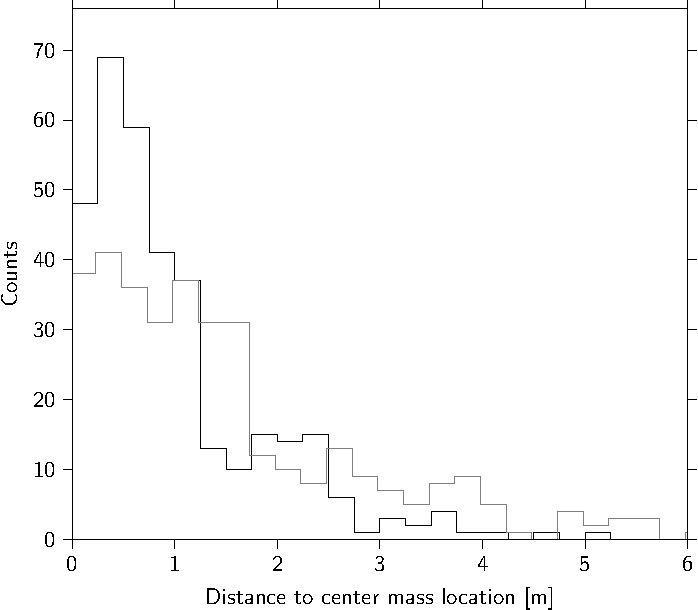
\includegraphics[width=0.6\textwidth]
                    {plots/cluster/gps_distance_cm_all}
    \caption{Station \gps location distances to station average location. For each station the results of multiple self-surveys are compared to their average location. The horizontal (black) and vertical (gray) distance distributions are shown.}
    \label{fig:gps_distance_cm_all}
\end{figure}

% What causes the size of the position error. High DOP because satellites always on Southern part of sky.
The size of the errors is partially due to the high latitude (\SI{>50}{\degree}) of the Netherlands. \gps satellite orbits are inclined by \SI{55}{\degree} relative to the Earth's equator. Rarely will a \gps satellite be seen straight overhead or towards the northern sky in the Netherlands. Most of the observed satellites will be on the southern part of the sky. For locations above \SI{55}{\degree} latitude \gps satellites always appear on the southern part of the sky. An elevation mask is used to exclude \gps satellites when they are within \SI{10}{\degree} of the horizon. This is done because signals from those satellites pass through a larger amount atmosphere, increasing the chances of distortions.

% GPS and detector locations. For example all GPS locations for 501. Detectors only moved once, need relative locations to GPS.
Station 501 has had five different physical \gps antenna locations, shown in \cref{fig:station_501_4D}. Two of these (the bottom and left one) are temporary locations which were used because the actual \gps antenna was being used for testing purposes. The two center positions are the new \gps locations for stations 501 and 510. Both are shown because the \gps antennae were switched between the two for a test. The actual scintillator detectors for station 501 were only moved once during operation. In \cref{fig:4d_station_501_detectors} these two detector layouts are shown. For each physical \gps location the relative scintillator detector positions have been measured.

\begin{figure}
    \centering
    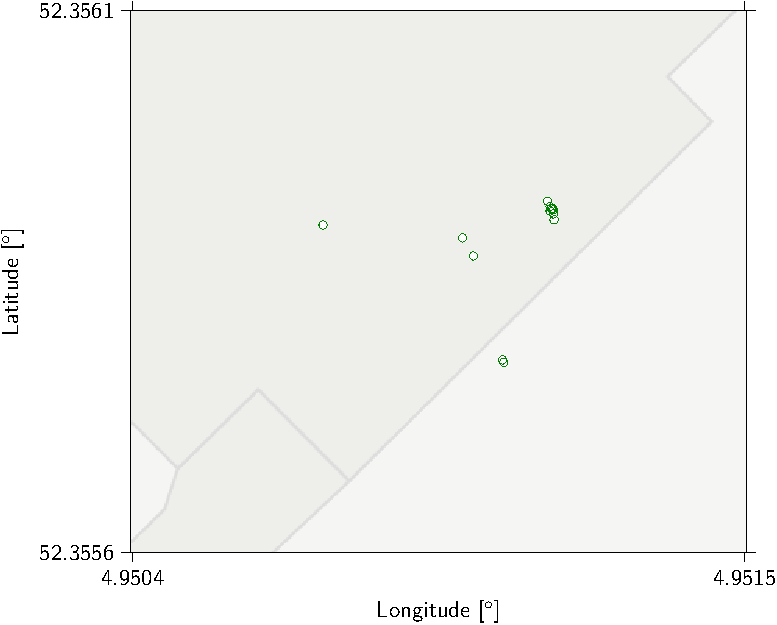
\includegraphics[width=0.6\textwidth]
                    {plots/cluster/station_501_4D}
    \caption{\gps locations reported by station 501 since starting data taking. At several point in time a different \gps antennae was used, and at times the antenna was moved. the closely spaced group of circles on the right are the same \gps antenna and location, the differences are caused by the different results from self-surveys.}
    \label{fig:station_501_4D}
\end{figure}


\section{Obtaining accurate absolute timestamps}

The \gps receiver is set in `Overdetermined Clock' mode after its position is determined to provide accurate timing. In this mode the \gps receiver keeps the position fixed and only concerns itself with timing. With the position of the \gps antenna fixed and the orbits of each \gps satellite known the current time can be determined with the signal of a single \gps satellite. However, when more satellite signals are used a more accurate result is achieved. According to the specifications this should result in an absolute timing accuracy of \SI{5}{\ns} \cite{trimble2007resolutiont}.


\subsection{Making event timestamps}
\label{sub:gps_timestamps}

% Explain what goes into creating an extended timestamp, from trigger and PPS to ext_timestamp.
Every second the \gps receiver sends a Pulse Per Second (\pps) signal to the \hisparc electronics to indicate the start of a second \cite{verkooijen2008firmware}. The \hisparc box uses a \SI{200}{\mega\hertz} clock to determine the time within this second. The clock is synchronised to the \pps by resetting its counter. However, the crystal in this internal clock does not work at exactly \SI{200}{\mega\hertz}. To correctly determine the time within a second the clock counter is read at the moment of a trigger (\ctd) and when each \pps arrives (\ctp). With these counts the fraction of the second at which the trigger occurred can be determined. For increased accuracy for the signal arrival time two \adcs per channel are used, one of which reads the signal on the negative side of the clock pulse. Resulting in a \SI{400}{\mega\hertz} clock with \SI{2.5}{\ns} sampling.

% What are the errors on determining the ext_timestamp and how are some corrected for/minimized.
The \pps signals have time errors relative to the actual \gps seconds, of up to \SI{20}{\ns}. This error is caused by the manner in which the \pps is produced. The effect is that the fraction between \ctd and \ctp does not result in a very accurate sub-second part of the timestamp. The \gps module has an internal high-precision clock with a frequency of \SI{12.504}{\mega\hertz}. The \pps is synchronised to the closest tick of this clock, of which both the positive and negative sides are used, resulting in the $(\SI{12.504}{\mega\hertz} \times 2 \times 2)^{-1} = \SI{\pm 20}{\ns}$. The size of this error is reported by the \gps module to the electronics after the \pps, this is called the Quantization error ($\Delta t_{\mathrm{Q}}$). This error is present at the start of each second, therefore both the error at the start ($\Delta t_{\mathrm{Q1}}$) and the end ($\Delta t_{\mathrm{Q2}}$) of a second are corrected. The total time between two \pps (i.e. the real time length represented by \ctp) is then $(10^9 - \Delta t_{\mathrm{Q1}} + \Delta t_{\mathrm{Q2}}) \si{\ns}$. Finally a synchronisation error ($\Delta t_{\mathrm{Sync}}$) between the \pps and the \hisparc clock exists. If the \pps arrived on the negative edge of the \SI{200}{\mega\hertz} clock the time needs to be shifted by \SI{2.5}{\ns}. Determination of the event timestamp is then done with the following equation
%
\begin{equation}
\label{eq:timestamp}
   \mathrm{Time[\si{\ns}]} =
      (S_n + 1) \cdot 10^9 +
      \Delta t_{\mathrm{Sync}} + \Delta t_{\mathrm{Q1}} +
      \left(\frac{\ctd}{\ctp}\right) \cdot
      \left(10^9 - \Delta t_{\mathrm{Q1}} + \Delta t_{\mathrm{Q2}}\right) \ ,
\end{equation}
%
here $S_n$ is the UNIX timestamp attached to an event in seconds. And example indicating these values and errors for a single \gps second is shown in \cref{fig:event_time}.

\begin{figure}
    \centering
    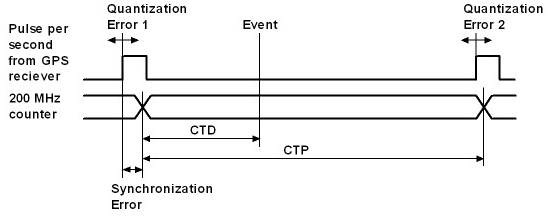
\includegraphics[width=0.6\textwidth]
                    {plots/cluster/event_time}
    \caption{Timeline of the values and errors required to determine the timestamp of an event. When The \pps from the \gps receiver arrives the \SI{200}{\mega\hertz} clock counter is reset. The \pps is offset from the real \gps second by $\Delta t_{\mathrm{Q}}$, this is also the case for the end of the second. The $\Delta t_{\mathrm{Sync}}$ indicates which side of the clock latched the \pps. The \ctd are the clock counts since the \pps until the trigger. \ctp is the number of clock counts between two \pps.}
    \label{fig:event_time}
\end{figure}

% Why the one second offset in messages. What data is contained in which message.
The value of $S_n$ is offset by one second from the actual \gps time. This is due to the order of messages from the \hisparc electronics. At the start of each second, when the \pps is recieved from the \gps module, the \hisparc electronics send a one second message (\osm) to the PC. These messages contain the \ctp, the date and time, the quantization error of the previous second, and also the synchronisation error of the current second. When a trigger occurs an event message is sent to the PC. This message contains the \ctd for the trigger, the date and time of the previous second, and the detector readouts. The reason that both the \osm and measured data messages contain the date and time of the previous second is that the \gps module sends the date and time of a second up to \SI{20}{\milli\second} after the \pps, in a message called the Primary Timing Packet \cref{trimble2009guide}. Between the \pps and the Primary Timing Packet multiple events may be triggered. In this time the electronics does not know the date and time of the current second yet. In order to be able to quickly empty the buffer for new events the date and time of the previous second are used instead of waiting. The electronics can not easily compute the date and time of the new second because incrementing the second might require incrementing the date. Date incrementation can be complicated due to different number of days per month and leap years. However, once the date has been converted to a UNIX timestamp on te PC incrementing the timestamp by one second is trivial. The date and time of the messages is used to find those that belong together. Events in a second belong to the second which was started with a \osm with the same date and time. This \osm contains the required synchronization error. The following two \osm are also required for the \ctp of the second and the Quantization errors. Note the Trimble user guide \cref{trimble2009guide} incorrectly states the quantization error value to be in seconds, the actual units are nanoseconds.

% Quickly send messages to empty the buffer, full buffer unlikely under normal conditions.
Events are sent to the PC as soon as possible to quickly empty the buffer to make space for subsequent triggers. The buffer can hold upto \SI{30}{\us} of data, i.e. five events with the default \SI{6}{\us} event length. If the trigger rate is much higher than the USB polling and transfer rate of the PC the buffer could fill up causing events to be lost. However, the probability of this occurring under normal data taking conditions is extremely low. Tests show that a trigger rate of \SI{30}{\hertz} can be sustained. The normal event rate of a station in opperation is only \SI{0.6}{\hertz}.


\subsubsection{Slave electronics timing}

% How it works for master/slave
The same timestamp calculation procedure is performed for events from the Master and Slave electronics, each sends their own \osm and measured data messages to the PC. The Master passes the received \pps from the \gps on to the Slave electronics. This synchronises their clocks, but also introduces another synchronisation error. The timestamps determined for the Master and Slave event are used to find which events belong together. After this they are simply combined, discarding the timing information from the Slave events. Due to the clock synchronisation errors between the Master and Slave errors of \SI{2.5}{\ns} between them are expected. This explains the time differences reported in \cref{sec:master_slave_timing}.


\subsection{Timestamp offsets}
\label{sec:gps_accuracy}

% Why we started \gps offset tests
An unexpected time offset between event timestamps was observed in a test where two \hisparc stations (501 and 502) were triggered by the same pulse generator \cite[p. 47]{fokkema2012hisparc}. Because these two stations separated by only $\sim\SI{90}{\meter}$ a narrow time difference distribution centered around \SI{0}{\ns} was expected. The standard deviation of the measured distribution was \SI{3}{\ns}, which is within the expected \gps accuracy of \SI{<5}{\ns}. However, a relatively large offset of \SI{18}{\ns} was seen. Further experiments with simultaneously triggered \hisparc electronics have been performed to find the sources contributing to this offset. Both the \hisparc electronics and \gps antennae are found to contribute to the offsets in event timestamps. The test setup and results will be discussed in the following sections.

The accuracy of the timing is examined to check consistency with the hardware specification. First the simple setup of two stations with only Master electronics is compared. Then the effects of adding Slave electronics and usage of the external trigger are checked. The effects of bad antenna position information is also determined.


\subsection{Timing accuracy test setup}
\label{sub:gps_test_setup}

% Describe the test setup.
In the setup the \hisparc electronics with hardware serial 62 is used as the reference point for the entire test. All other \hisparc boxes were tested against this reference, one at a time. Two \gps antennae separated by \SI{18}{\meter} and a \gps splitter \ref{gps2015splitter} were used. With the splitter tests could be performed in which both \hisparc electronics used the same \gps antenna, removing the offset caused by using different \gps antennae. A pulse generator \ref{tabor2005pulsegenerator}, with two short equal-length signal cables and a signal splitter was used to trigger the \hisparc electronics using the \pmt signal inputs. The electronics were set to trigger on a single high signal. In \cref{fig:setup} the setup is schematically shown. For every trigger the timestamps reported by the reference and the test subject were compared to get the offset and spread.

\begin{figure}
    \centering
    \tikzsetnextfilename{externalized-gps_test_setup}
 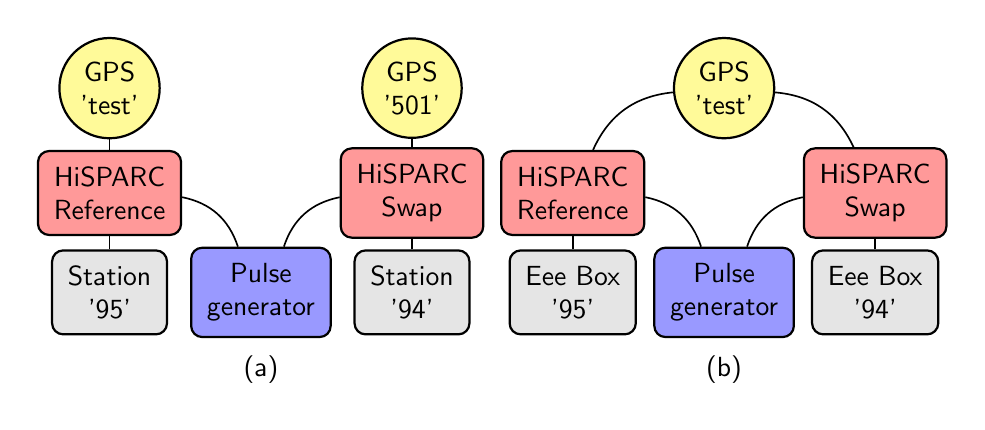
\begin{tikzpicture}
  [font=\sffamily,
   every matrix/.style={ampersand replacement=\&,column sep=0.1cm,row sep=0.1cm},
   gps/.style={draw,thick,circle,fill=yellow!40,inner sep=.1cm, align=center},
   pc/.style={draw,thick,rounded corners,fill=black!10,inner sep=.2cm, align=center},
   hisparc/.style={draw,thick,rounded corners,fill=red!40,inner sep=.2cm, align=center},
   pulse/.style={draw,thick,rounded corners,fill=blue!40,inner sep=.2cm, align=center},
   to/.style={-,semithick,font=\sffamily\footnotesize},]

  \matrix{
   \node[gps] (test) {GPS\\'test'}; \& \& \node[gps] (501) {GPS\\'501'}; \& \& \& \node[gps] (b_test) {GPS\\'test'}; \& \\
   \node[hisparc] (refr) {HiSPARC\\Reference}; \& \& \node[hisparc] (swap) {HiSPARC\\Swap}; \& \& \node[hisparc] (b_refr) {HiSPARC\\Reference}; \& \& \node[hisparc] (b_swap) {HiSPARC\\Swap}; \\
   \node[pc] (95) {Station\\'95'}; \& \node[pulse] (pulse) {Pulse\\generator}; \& \node[pc] (94) {Station\\'94'}; \& \& \node[pc] (b_95) {Eee Box\\'95'};  \& \node[pulse] (b_pulse) {Pulse\\generator}; \& \node[pc] (b_94) {Eee Box\\'94'}; \\
   \& \node {(a)}; \& \& \& \& \node {(b)}; \& \\
  };
  
  \draw[to] (test) -- node[below,above,sloped] {} (refr);
  \draw[to] (501) -- node[below,above,sloped] {} (swap);
  \draw[to] (95) -- node[midway,midway,sloped] {} (refr);
  \draw[to] (94) -- node[midway,midway,sloped] {} (swap);
  \draw[to] (pulse) to[bend left] node[above,below,sloped] {} (swap);
  \draw[to] (pulse) to[bend right] node[above,below,sloped] {} (refr);

  \draw[to] (b_test) to[bend right] node[below,above,sloped] {} (b_refr);
  \draw[to] (b_test) to[bend left] node[below,above,sloped] {} (b_swap);
  \draw[to] (b_95) -- node[midway,midway,sloped] {} (b_refr);
  \draw[to] (b_94) -- node[midway,midway,sloped] {} (b_swap);
  \draw[to] (b_pulse) to[bend left] node[above,below,sloped] {} (b_swap);
  \draw[to] (b_pulse) to[bend right] node[above,below,sloped] {} (b_refr);

 \end{tikzpicture}

    \caption{This image shows the two setups of the test. Two station PCs are used to control the \hisparc Master electronics (Reference and Test). The electronics are triggered simultaneously by same pulse generator. Each is also connected to a \gps antenna, some tests used separate \gps antennae (a) and in some tests the same \gps antenna was used by both via the splitter (b).}
    \label{fig:setup}
\end{figure}

% Explain why the data taken immediately after power on is not valid, wait for ephemeris/almanac.
When the test subject was connected to the \gps antenna the position of the antenna was given to the \gps module. Most of the tested electronics had not been connected to power for considerable time and therefore didn't have the current ephemeris data. This causes errors in the calculation of \gps satellite orbits, which translate into errors in the timestamps. An example of a jump in timing precision due first missing and at some point retrieving ephemeris data is shown in \cref{fig:tt_delta_time_074}. At the start of this test a cold reset was performed. In a cold reset the almanac and ephemeris data is cleared from the \gps receiver. To prevent influence from this the first part of each test is excluded.

\begin{figure}
    \centering
    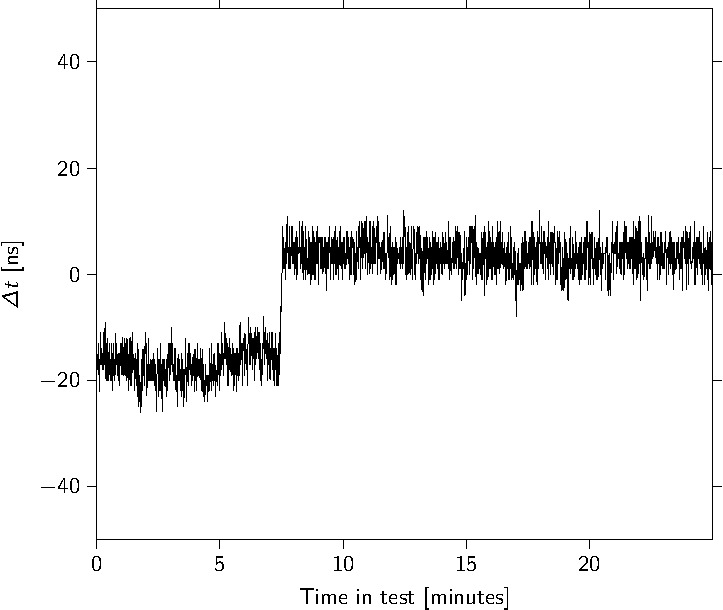
\includegraphics{plots/cluster/tt_delta_time_074}
    \caption{Time difference between test electronics and the reference versus time of the test. Several minutes into the test a jump can be seen. That is when the ephemeris data is obtained.}
    \label{fig:tt_delta_time_074}
\end{figure}


\subsection{Results of time offset and accuracy tests}
\label{sub:gps_offsets}

% Summary of the tests
In total 32 tests were performed, 10 tests with the setup shown in \cref{fig:setup}a and 22 tests with the setup \cref{fig:setup}b. Each test was with a different \hisparc electronics unit for the `Test' station. Besides these 32 tests, additional tests with different configurations were performed. These include Master-Slave combinations, using the external trigger, or using intentionally offset \gps positions.

% Summary of results from normal tests
In the tests with separate \gps antennae the average offset was around \SI{25}{\ns}. Swapping the \gps antennae between the two electronics resulted in an offset shift of \SI{16}{\ns}. When using the splitter the average offset was only \SI{1.8}{\ns}. This indicates that the different \gps antennae and cables are a large source of offsets. The different \hisparc electronics also contribute to the offset, the standard deviation of the offsets is \SI{2.7}{\ns}. Also the average standard deviation of the time difference distributions of the tests decreased from \SI{4.7}{\ns} to \SI{3.2}{\ns} [double check these values] when using the splitter instead of separate antennae. The achieved timing accuracies are within the specification, except for the offsets. The results of the tests are shown in \cref{fig:tt_offset_Good}. The cause for the outliers is unclear.

\begin{figure}
    \centering
    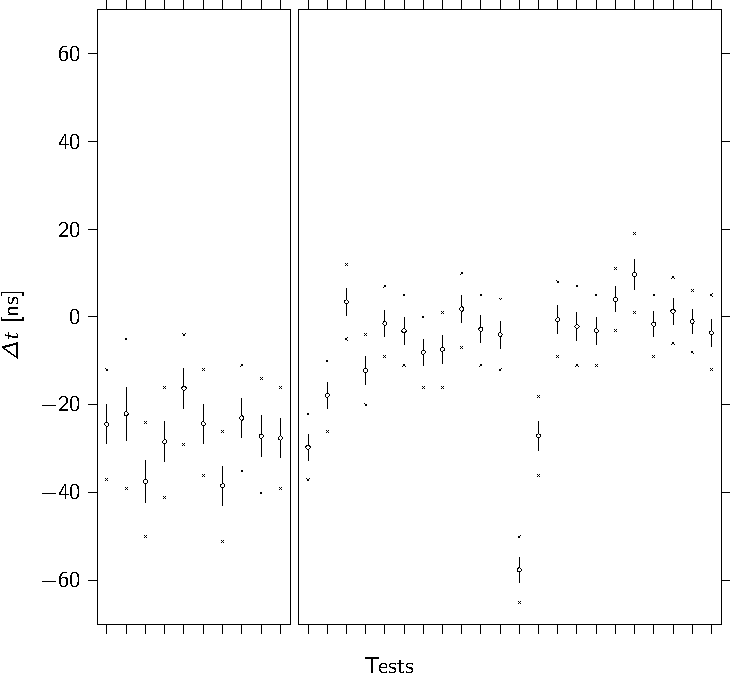
\includegraphics[width=0.6\textwidth]
                    {plots/cluster/tt_offset_Good}
    \caption{Time offsets test results. The mean offset (circles) are shown with the standard deviation (error bars) and the minimum and maximum time differences (crosses). The results from tests with separate \gps antennae (left panel) and those with the splitter (right panel) are shown.}
    \label{fig:tt_offset_Good}
\end{figure}


\subsubsection{Effects of alternative triggering}

% Effect of using a Slave. Effect of using the external trigger.
Tests were performed with a Slave attached to the electronics of the Test station. The signal input was connected to the Slave to see if the offset was affected. The resulting offsets where within \SI{2.5}{\ns} of the test with the same Master without the Slave. In several tests the input was switched from the regular \pmt inputs to the external trigger. The expected offsets \cref{sssec:external-trigger} in the \gps timestamps were seen, and the accuracy of the timing remained equal.


\subsubsection{Wrong position leads to inaccurate timing}

% Effect of wrong position in the GPS receiver. Greater the offset the lower the accuracy. If the offset is to large the GPS automatically performs a self-survey.
In several tests a bad position was entered in the \gps module. This made the \gps receiver think the \gps antenna was placed a certain distance away from the actual antenna position. The timing accuracy degraded as a result. Moreover, the time differences over time showed clear \SI{24}{\hour} periodicity. The results of these tests is shown in \cref{fig:tt_delta_time_89_22_44_3}. The width of the time difference distribution increase with the position offset. For the shown tests the standard deviations are \SIlist{3.3;11.9;16.4;>66}{\ns}, corresponding to the position offsets of \SIlist{0;25;55;100}{\meter}. For the expected position error of up to \SI{2}{\meter} the timing accuracy should still be excellent. If a \gps module is given a position more than \SI{250}{\meter} from its actual position a self-survey will automatically be started to acquire a better position.

\begin{figure}
    \centering
    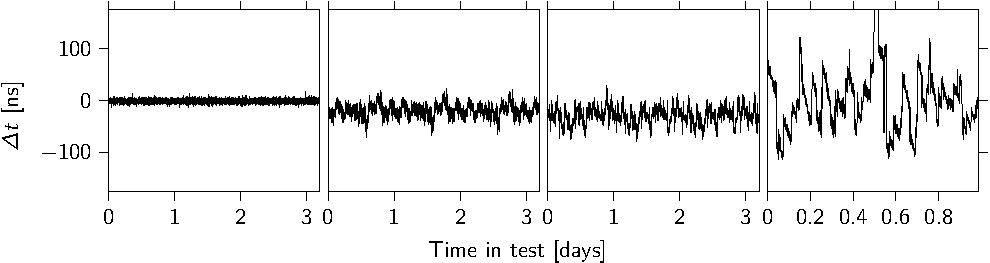
\includegraphics[width=\textwidth]
                    {plots/cluster/tt_delta_time_89_22_44_3}
    \caption{Time difference measurements for tests where a \gps was given wrong position information. From left to right the position offsets are \SIlist{0;25;55;100}{\meter}. The errors in the time offset vary during the day and clearly follow a \SI{24}{\hour} period, most clear in the second panel. This is the period at which \gps satellite configurations on the sky repeat. In the last panel large sudden jumps can be seen, these probably occur when the \gps receiver selects a different \gps satellite as primary time source.}
    \label{fig:tt_delta_time_89_22_44_3}
\end{figure}


\section{The \hisparc network}

\subsection{Station locations}

% Current station locations, explain why the stations are in those locations. Due to those being the locations of high schools..
In \cref{fig:network_weather_knmi} the locations of all \hisparc stations is shown. In 2004 \hisparc started data collection. Initially with several stations in Amsterdam, then expanding to other regions. Presently there are over \num{120} active \hisparc stations collecting data. Most stations are clustered in or around large cities. Almost all stations are located at high schools and universities. Universities provide support for the high schools in their region, they guide students in building the scintillator detectors and provide assistance when needed. There are \num{70} Dutch high schools participating in \hisparc. This is more than \SI{10}{\percent} of the total number of high schools in the Netherlands \cite{duo2016hoofd}.

\begin{figure}
    \centering
    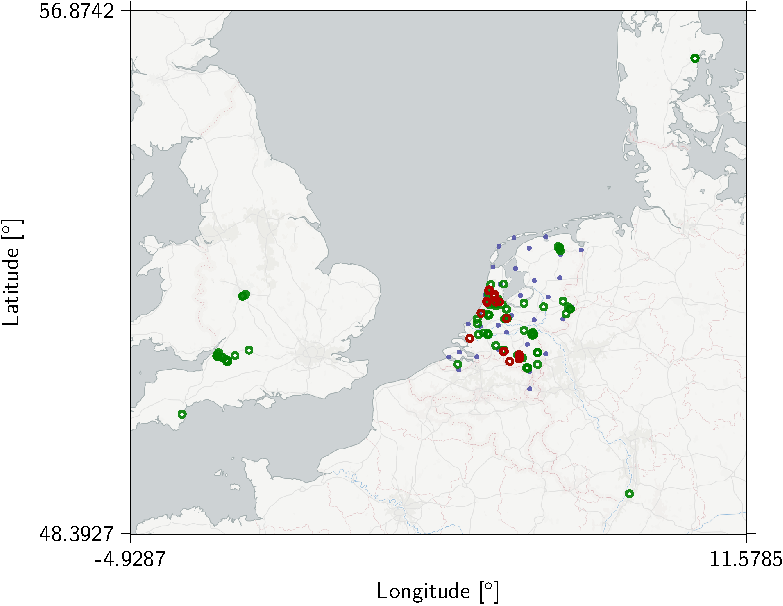
\includegraphics[width=0.6\textwidth]
                    {plots/cluster/network_weather_knmi}
    \caption{Locations of \hisparc stations in Netherlands, United Kingdom, and Denmark. Stations which also include a weather station are indicated with red circles. The Dutch \knmi stations are indicated in blue.}
    \label{fig:network_weather_knmi}
\end{figure}


\subsubsection{The Science Park cluster}

The largest group of clustered stations in the \hisparc network is at the Science Park in Amsterdam. This is where \nikhef is located and \hisparc is coordinated from. There are 11 4-detector stations at the Science Park. For all Science Park stations the detector positions are accurately known. In \cref{fig:subcluster_500} the detectors positions are shown. Half of the stations are placed in or have been rearanged to the diamond layout. This cluster will be extensively used in the analysis presented in this thesis.

\begin{figure}
    \centering
    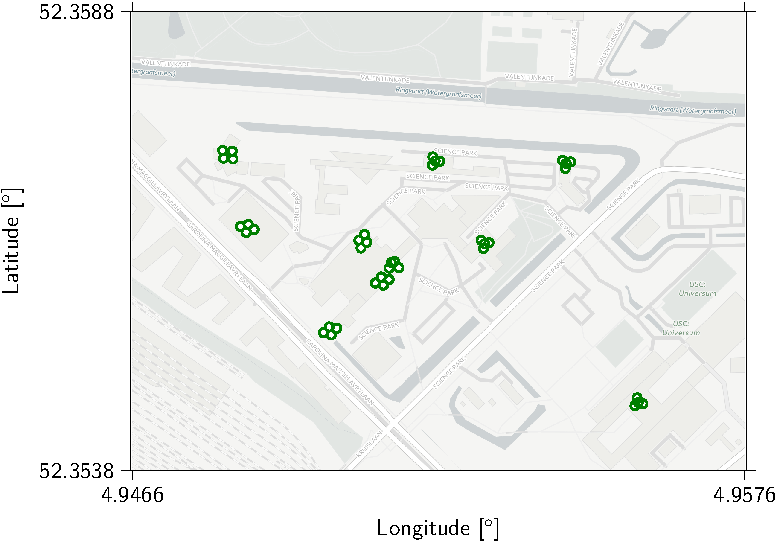
\includegraphics[width=0.6\textwidth]
                    {plots/cluster/subcluster_500}
    \caption{The Science Park scintillator detector locations. This shows the positions of stations 501 through 511.}
    \label{fig:subcluster_500}
\end{figure}


\subsubsection{International}

% Locations in other countries
Locations of \hisparc stations are not limited to the Netherlands. Two other countries also successfully operate multiple detection stations.

Since 2007 there has been a \hisparc station in Denmark. There are currently 3 operational stations at the Aarhus University. In the United Kingdom a cluster was formed around Bristol in 2012. Since then more than 10 schools around Bristol have build detection stations and joined the network. Even more schools have plans to join. In 2014 a second cluster was started in the United Kingdom around Birmingham.

In Germany a station (70001) was placed inside the \kascade experiment in Karlsruhe. The station operated there from 2008 up to and including 2011. This was done to calibrate and test the reconstruction accuracy of a single \hisparc station, as reported in [ref previous chap]. Although the \kascade-Grande experiment officially shut down on March 30, 2009, the detectors were kept active until November, 26th 2011 as a test facility for other experiments. When the \kascade detectors detected a shower the \hisparc station was triggered using the external trigger. The detectors used for the \kascade station have since been reused and now form a station (508) at the Science Park.


\subsection{Uptime}

% Timeline of number of active stations. Explain why stations may be down, i.e. why less are up than 'active'.
Unfortunately not all stations continue to operate properly. \cref{fig:active_stations} shows the cumulative number of stations that have had at least two consecutive days of events and the number of active stations per week. Over the last \SI{12}{\year} the number of detection stations with data has grown at an average rate of one per month. The number of active stations also increases but lags behind the total number of stations. Stations permanently going offline has been taken into account, subtracting them the active stations when they stopped taking data [Todo, ~8 stations]. In some cases the contact person at a high station retired without arranging followup, leaving the station without proper maintenance. Other problems that have been known to cause stations to be down are Windows Updates, internet connectivity, bad configuration, power supply failures, light leaks in the detectors, or some other issues \cite{delaat2013maintenance}. In many cases (software or configuration related problems) remote control of the station can be used to make station operational again.

\begin{figure}
    \centering
    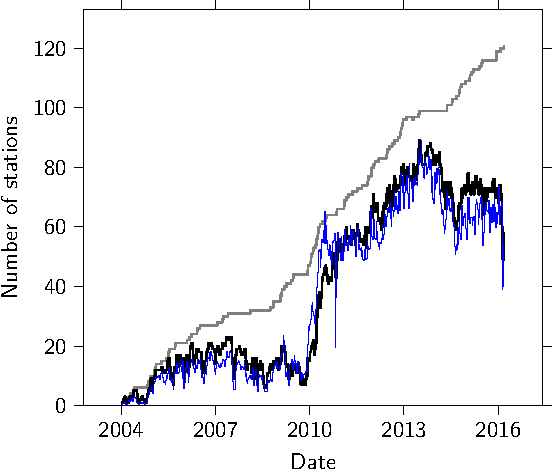
\includegraphics[width=0.6\textwidth]
                    {plots/cluster/active_stations}
    \caption{Cumulative number of stations with at least two consecutive days of data and the number of active stations per day.}
    \label{fig:active_stations}
\end{figure}

% Each station submits data/triggered events to central datastore
Recorded events are uploaded to the central datastore at \nikhef. Here further offline analysis is performed and the data is made available for download. The automatic data analysis that is performed is described in [a later chapter]. The data is sent from the station to the datastore server. The server verifies the request and stores the data in the raw datastore. The datastore stores the detected events, configuration settings, error messages, single rates, and \gps signal information. Additionally a station may upload weather data, for which the data, configuration, and errors are stored. In \cref{fig:luminosity_network} the cumulative number of detected events is shown.

\begin{figure}
    \centering
    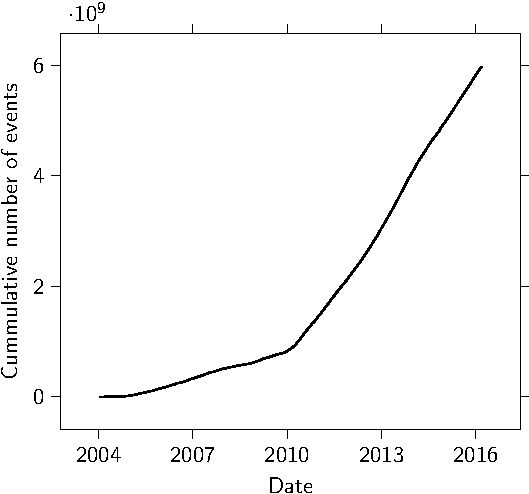
\includegraphics[width=0.6\textwidth]
                    {plots/cluster/luminosity_network}
    \caption{Cumulative number of events by all stations.}
    \label{fig:luminosity_network}
\end{figure}

% Use offline analysis to find station events detecting the same shower.
  % - This requires good absolute timing at the stations.
  % - Use GPS at stations for both positioning of the stations (\SI{~1}{\meter}) and absolute timing (\SI{~5}{\ns}).
The data from multiple \hisparc stations can be combined to perform shower reconstruction with more detection points than a single station and separated by larger distances. In order to combine the data the exact detection time of  detected showers must be known. The \gps receiver provides the accurate timestamp. An `offline trigger' is used to determine when stations were probably detecting the same shower. The data is searched for (at least two) stations that simultaneously (i.e. within \SI{10}{\us}) detected events. Coincidences between stations are expected to be caused by either the detection of the same shower, the detection of separate but correlated showers (e.g. the GZ-effect), or the detection of two unrelated showers. The accuracy of the timing influences the resolution with which shower reconstruction can be performed. The \gps module provides accurate timestamps if the position is properly calibrated.

Important for shower reconstruction, coincidence rate, and possibilities for detection the GZ-effect are the distances between pairs of stations. In \cref{fig:station_distances_all} the distribution of distances between all possible pairs of stations are shown. The points beyond \SI{250}{\kilo\meter} are due to combinations between stations in different countries. And the pair separated by only \SI{2}{\meter} is the combination of station 501 and 510. These were intentionally interlaced to compare the results from two stations which are virtually at the same location. The results from comparing these stations is shown in [ref to later chapter about station performance or reconstructions].

\begin{figure}
    \centering
    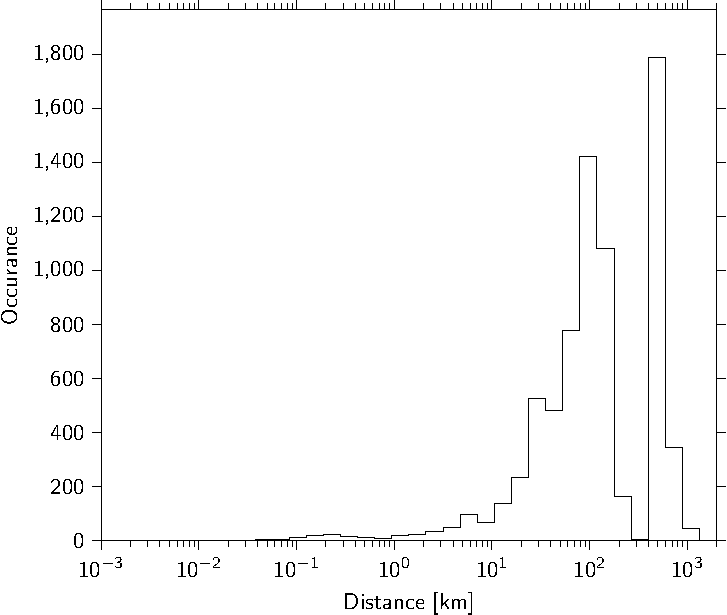
\includegraphics[width=0.6\textwidth]
                    {plots/cluster/station_distances_all}
    \caption{Distribution of distances between all possible pairs of stations in the entire \hisparc network.}
    \label{fig:station_distances_all}
\end{figure}


\section{Detection by multiple stations}
\label{sec:detection-multiple-stations}

% Stations closer than \SI{2e3}{\meter} are likely to at some point detect the same shower.
Station pairs separated by up to \SI{2e3}{\meter} occasionally detect the same shower at some point in time. At distances of \SI{2e3}{\meter} the rate of coincidences is close to the rate of random coincidences due to the event rate of the individual stations. Real events may still be distinguishable from background if the event can be reconstructed. Large showers which can be detected efficiently by two stations both \SI{e3}{\meter} from the shower core have energies of at least \SI{e18}{\eV}. Such showers are rare, from \cref{fig:spectrum} we can estimate a rate of approximately \SI{1}{\per\kilo\meter\squared\per\day}. The sensitivity to those showers is not equal over that \si{\kilo\meter\squared} area, so a lower rate is expected.

% estimate the coincidence rate for showers of certain energy.
As the distance between stations increase the probability of detecting low energy showers decrease. Meanwhile the probability of detecting high energy showers is low because of their low flux. The highest contributions to coincidences are the lowest energy showers that can just barely be detected efficiently. This smoothly transitions to continually higher showers being the dominant source for coincidences as the distances increases. A rough estimate of the coincidence rate can be made. For detector stations at a given distance calculate the probability of detecting showers for all relevant energies in the cosmic-ray spectrum (\SIrange{e13}{e20}{\eV}). Assume that the shower hit precisely between the stations, where the probability is highest. Scale the determined probability of detection with the occurrence of such showers and compensate for the larger effective area for which high energy showers will be detectable.

In \cref{fig:distance_v_coincidence_rate} the coincidence rate is determined for all pairs of stations which are closer than \SI{2e3}{\meter}. Only periods in which both stations were working properly are considered. The determined coincidence rate is then plotted against the distance between the stations. Different coincidence rates due to detection efficiencies caused by the different number of detectors in stations is expected. The different combinations of two 2-detector, two 4-detector, and a 2- and 4-detector stations are indicated by different symbols. The background rate is estimated by \cref{eq:background_rate} and indicated by the horizontal dashed lines. A set of station pairs too far apart (\SI{>9}{\kilo\meter}) to expect real coincidences from is also shown to verify the background rates.

\begin{figure}
    \centering
    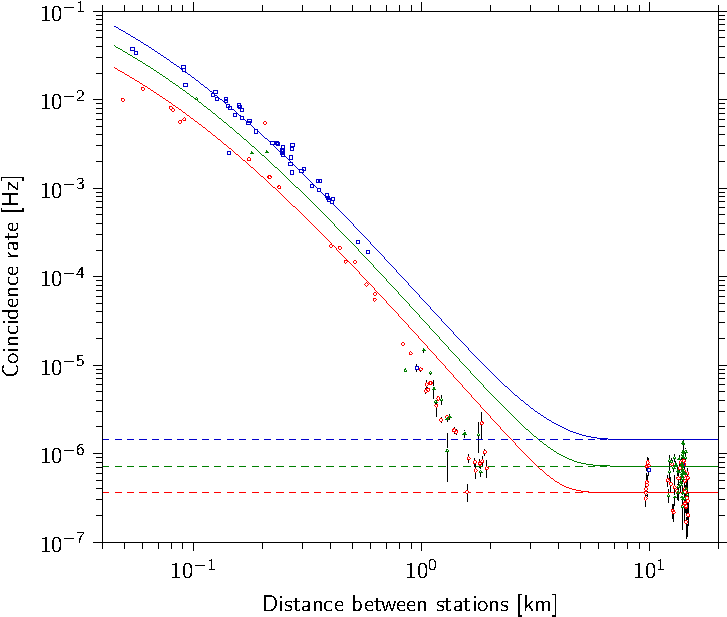
\includegraphics[width=0.6\textwidth]
                    {plots/cluster/distance_v_coincidence_rate}
    \caption{Coincidence rate between station pairs as a function of distance. Pairs of two 4-detector stations (squares, blue), a 4- and 2-detector station (triangle, green), and two 2-detector stations (circle, red) are shown. The expected coincidences rates, including background, are shown (solid). The background rate is also shown separately (dashed). At increasing distances the contributions from increasingly larger/energetic showers dominate, until the background takes over. [todo update for 10us window]}
    \label{fig:distance_v_coincidence_rate}
\end{figure}


\subsection{Compensating for \gps timing offsets}
\label{ssec:compensating_gps_offset}

The \gps time offset between stations can be determined from real data. For any combination of two stations the expected mean time difference of all coincident events is \SI{0}{\ns}, because of mirror symmetry. However, the width of the distribution is very dependent on the distance between the stations, because inclined showers will result in larger time differences if the stations are further apart, and a large core distances the effect of shower front curvature and rise time become more relevant. Moreover, the increased distance means that less events will be detected by both stations simultaneously because showers of higher energy and larger footprints occur less often. To determine the offset between stations that are further apart more data is required, and a longer time is required to get that data. However, as the distance between stations increases the time offsets become less important because the effect on the shower reconstruction will be less significant at the large distance.

The offsets were found to be stable over time and varying for different combinations of \hisparc electronics and \gps antennae. In some cases the offset was larger than \SI{30}{\ns}, which can have a significant effect on the direction reconstruction of showers, depending on the distance to other stations.

The \hisparc stations at the Amsterdam Science Park are relatively close. This results in a coincidence rate of at least 25 per day, for the two stations furthest apart. By collecting coincidences from multiple days enough data can be gathered to accurately determine the time offset between the stations. In \cref{fig:offsets_ref502_503_pairs} the offsets between station 502 and 503 is shown versus time. Most of the time the offset is stable but some jumps can be seen. Most of the significant jumps can be related to changes in the station components.

[Fix explanations]
%The large offset around 2012 is due to station 501 temporarily using a \gps antenna with bad sky coverage. Around 2013 the electronics were replaced by new versions. In 2015 station 501 was moved in a new configuration with station 510. Determining the moment of transition from one `offset' to the next is difficult due to the width of the time difference distributions.

\begin{figure}
    \centering
    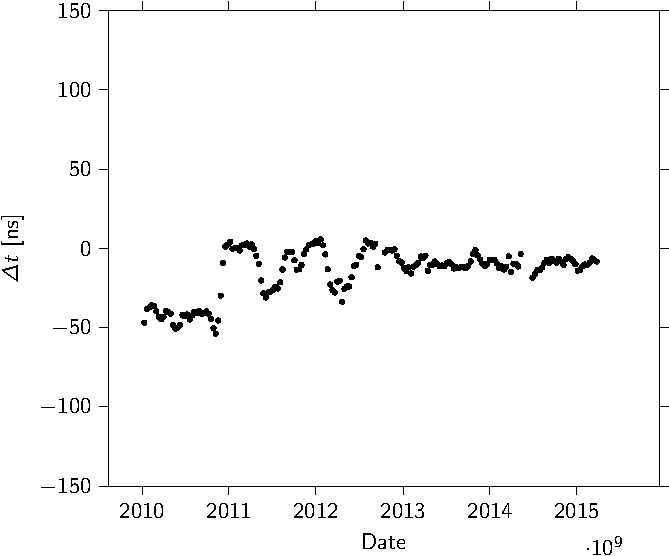
\includegraphics[width=0.6\textwidth]
                    {plots/cluster/offsets_ref502_503_pairs}
    \caption{\gps time offset between stations 502 and 503 versus time. For each point multiple days of data are used to accurately determine the offset. Changes of \SI{>50}{\ns} are seen. Most changes are due to changes in station components.}
    \label{fig:offsets_ref502_503_pairss}
\end{figure}

\begin{figure}
    \centering
    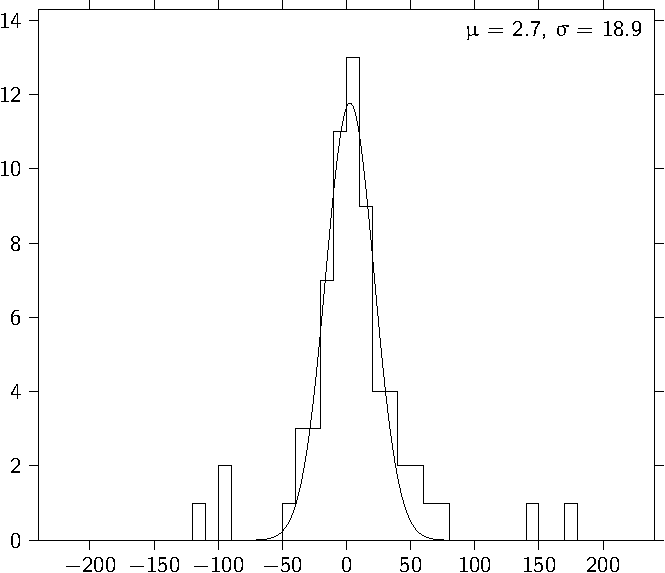
\includegraphics{plots/cluster/offset_distribution}
    \caption{Distribution of station offsets at a moment in time. The data is for 66 station pairs, many stations are included more than once. The distribution mean is close to 0, unfortunately fairly wide.}
    \label{fig:test_offset_distribution}
\end{figure}


\subsection{Time difference distribution}
\label{ssec:time-difference-distribution}

The time difference distributions used to determine the station offsets take into account that the trigger time (event timestamp) is not the arrival time of the first shower particle in the detectors. The trigger occurs when the second (or third) signal is detected. The time difference between the trigger time and first particle arrival time is subtracted from the event timestamp. Moreover, this time difference is also corrected for detector offsets, as described in \cref{sec:detector-offsets}.

A simple flat shower front simulation can be performed to predict the expected time difference distributions. This is only a time-based simulation, not a particle simulation, so the attenuation of inclined showers has to be accounted for when inputting showers. Here the $\sin \theta \cos^7 \theta$ distribution is used. This distribution should be shower energy dependent, because inclined low energy showers have a more difficult time to reach ground level than high energy showers. However, than is not taken into account in this case. This introduces a wider than expected distribution at short distances, because low energy showers tend to arrive from small zenith angles. And a narrower than predicted distribution at larger distances. In \cref{fig:dt_ref504_509_dist_sim} the time difference distribution of real data from station pair 504 and 509 is compared to the simulation. The stations are separated by \SI{305}{\meter}. The simulation accurately predicts the time difference distribution. A Normal distribution was also fit to the data. This does not fit well because the tails are shorted for the real data. This is partly because there is a maximum expected time difference equal to the time light takes to travel from one station to the other. In this case \SI{1017}{\ns}. This would be the extreme case of a horizontal air shower. Detector effects and shower rise time might cause even longer time differences, but horizontal showers are very rare to begin with.

\begin{figure}
    \centering
    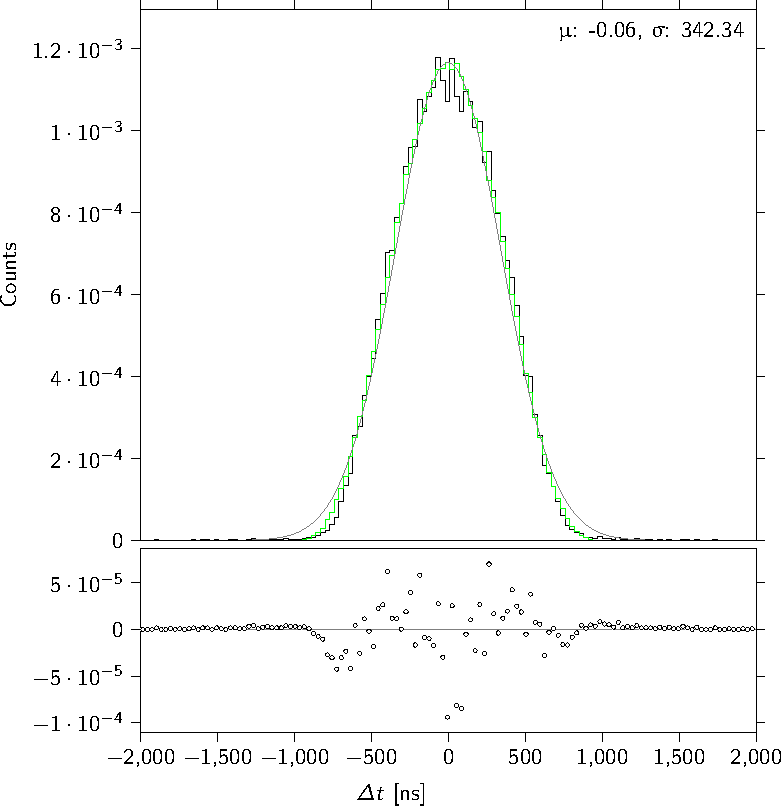
\includegraphics[width=0.6\textwidth]
                    {plots/cluster/dt_ref504_509_dist_sim}
    \caption{Arrival time distribution between stations (black) compared with simulated time distribution using a simple cone shaped shower front and the expected zenith distribution as input (green). The data and simulated distributions match well, residual differences may be due to shower front thickness or orther small effects that are not taken into account in the simulation. A fit by a Normal distribution (gray) does not accurately describe the data, shorter tails are seen.}
    \label{fig:dt_ref504_509_dist_sim}
\end{figure}

An correlation exists between the width of the time difference distribution and the distance between the stations. In \cref{fig:distance_v_width_sim} the widths of the pairs of Science Park stations is shown compared to the simulated widths for the same pairs. The simulation accurately predicts the width of the distributions. The residuals are due to the different zenith distributions which was not taken into account.

\begin{figure}
    \centering
    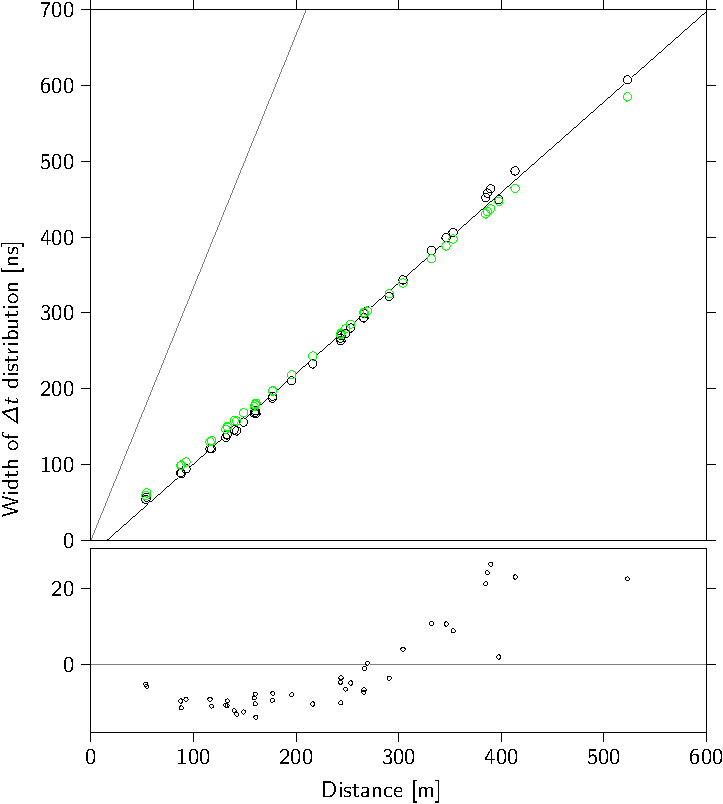
\includegraphics[width=0.6\textwidth]
                    {plots/cluster/distance_v_width_sim}
    \caption{Width of time difference distribution as function of distance between stations. Shown for real data (black) and for simulations (green). The distribution widens due to angled showers. Larger distance less low energy showers which have smaller angle acceptance. Zenith peak shifts to higher angles, increasing the width further. As a reference the expected maximum time difference is also indicated by the gray line.}
    \label{fig:distance_v_width_sim}
\end{figure}
